\documentclass[a4paper]{article}

\def\npart{II}

\def\ntitle{Graph Theory}
\def\nlecturer{I.\ Leader}

\def\nterm{Michaelmas}
\def\nyear{2018}

\ifx \nauthor\undefined
  \def\nauthor{Qiangru Kuang}
\else
\fi

\ifx \ntitle\undefined
  \def\ntitle{Template}
\else
\fi

\ifx \nauthoremail\undefined
  \def\nauthoremail{qk206@cam.ac.uk}
\else
\fi

\ifx \ndate\undefined
  \def\ndate{\today}
\else
\fi

\title{\ntitle}
\author{\nauthor}
\date{\ndate}

%\usepackage{microtype}
\usepackage{mathtools}
\usepackage{amsthm}
\usepackage{stmaryrd}%symbols used so far: \mapsfrom
\usepackage{empheq}
\usepackage{amssymb}
\let\mathbbalt\mathbb
\let\pitchforkold\pitchfork
\usepackage{unicode-math}
\let\mathbb\mathbbalt%reset to original \mathbb
\let\pitchfork\pitchforkold

\usepackage{imakeidx}
\makeindex[intoc]

%to address the problem that Latin modern doesn't have unicode support for setminus
%https://tex.stackexchange.com/a/55205/26707
\AtBeginDocument{\renewcommand*{\setminus}{\mathbin{\backslash}}}
\AtBeginDocument{\renewcommand*{\models}{\vDash}}%for \vDash is same size as \vdash but orginal \models is larger
\AtBeginDocument{\let\Re\relax}
\AtBeginDocument{\let\Im\relax}
\AtBeginDocument{\DeclareMathOperator{\Re}{Re}}
\AtBeginDocument{\DeclareMathOperator{\Im}{Im}}
\AtBeginDocument{\let\div\relax}
\AtBeginDocument{\DeclareMathOperator{\div}{div}}

\usepackage{tikz}
\usetikzlibrary{automata,positioning}
\usepackage{pgfplots}
%some preset styles
\pgfplotsset{compat=1.15}
\pgfplotsset{centre/.append style={axis x line=middle, axis y line=middle, xlabel={$x$}, ylabel={$y$}, axis equal}}
\usepackage{tikz-cd}
\usepackage{graphicx}
\usepackage{newunicodechar}

\usepackage{fancyhdr}

\fancypagestyle{mypagestyle}{
    \fancyhf{}
    \lhead{\emph{\nouppercase{\leftmark}}}
    \rhead{}
    \cfoot{\thepage}
}
\pagestyle{mypagestyle}

\usepackage{titlesec}
\newcommand{\sectionbreak}{\clearpage} % clear page after each section
\usepackage[perpage]{footmisc}
\usepackage{blindtext}

%\reallywidehat
%https://tex.stackexchange.com/a/101136/26707
\usepackage{scalerel,stackengine}
\stackMath
\newcommand\reallywidehat[1]{%
\savestack{\tmpbox}{\stretchto{%
  \scaleto{%
    \scalerel*[\widthof{\ensuremath{#1}}]{\kern-.6pt\bigwedge\kern-.6pt}%
    {\rule[-\textheight/2]{1ex}{\textheight}}%WIDTH-LIMITED BIG WEDGE
  }{\textheight}% 
}{0.5ex}}%
\stackon[1pt]{#1}{\tmpbox}%
}

%\usepackage{braket}
\usepackage{thmtools}%restate theorem
\usepackage{hyperref}

% https://en.wikibooks.org/wiki/LaTeX/Hyperlinks
\hypersetup{
    %bookmarks=true,
    unicode=true,
    pdftitle={\ntitle},
    pdfauthor={\nauthor},
    pdfsubject={Mathematics},
    pdfcreator={\nauthor},
    pdfproducer={\nauthor},
    pdfkeywords={math maths \ntitle},
    colorlinks=true,
    linkcolor={red!50!black},
    citecolor={blue!50!black},
    urlcolor={blue!80!black}
}

\usepackage{cleveref}



% TODO: mdframed often gives bad breaks that cause empty lines. Would like to switch to tcolorbox.
% The current workaround is to set innerbottommargin=0pt.

%\usepackage[theorems]{tcolorbox}





\usepackage[framemethod=tikz]{mdframed}
\mdfdefinestyle{leftbar}{
  %nobreak=true, %dirty hack
  linewidth=1.5pt,
  linecolor=gray,
  hidealllines=true,
  leftline=true,
  leftmargin=0pt,
  innerleftmargin=5pt,
  innerrightmargin=10pt,
  innertopmargin=-5pt,
  % innerbottommargin=5pt, % original
  innerbottommargin=0pt, % temporary hack 
}
%\newmdtheoremenv[style=leftbar]{theorem}{Theorem}[section]
%\newmdtheoremenv[style=leftbar]{proposition}[theorem]{proposition}
%\newmdtheoremenv[style=leftbar]{lemma}[theorem]{Lemma}
%\newmdtheoremenv[style=leftbar]{corollary}[theorem]{corollary}

\newtheorem{theorem}{Theorem}[section]
\newtheorem{proposition}[theorem]{Proposition}
\newtheorem{lemma}[theorem]{Lemma}
\newtheorem{corollary}[theorem]{Corollary}
\newtheorem{axiom}[theorem]{Axiom}
\newtheorem*{axiom*}{Axiom}

\surroundwithmdframed[style=leftbar]{theorem}
\surroundwithmdframed[style=leftbar]{proposition}
\surroundwithmdframed[style=leftbar]{lemma}
\surroundwithmdframed[style=leftbar]{corollary}
\surroundwithmdframed[style=leftbar]{axiom}
\surroundwithmdframed[style=leftbar]{axiom*}

\theoremstyle{definition}

\newtheorem*{definition}{Definition}
\surroundwithmdframed[style=leftbar]{definition}

\newtheorem*{slogan}{Slogan}
\newtheorem*{eg}{Example}
\newtheorem*{ex}{Exercise}
\newtheorem*{remark}{Remark}
\newtheorem*{notation}{Notation}
\newtheorem*{convention}{Convention}
\newtheorem*{assumption}{Assumption}
\newtheorem*{question}{Question}
\newtheorem*{answer}{Answer}
\newtheorem*{note}{Note}
\newtheorem*{application}{Application}

%operator macros

%basic
\DeclareMathOperator{\lcm}{lcm}

%matrix
\DeclareMathOperator{\tr}{tr}
\DeclareMathOperator{\Tr}{Tr}
\DeclareMathOperator{\adj}{adj}

%algebra
\DeclareMathOperator{\Hom}{Hom}
\DeclareMathOperator{\End}{End}
\DeclareMathOperator{\id}{id}
\DeclareMathOperator{\im}{im}
\DeclarePairedDelimiter{\generation}{\langle}{\rangle}

%groups
\DeclareMathOperator{\sym}{Sym}
\DeclareMathOperator{\sgn}{sgn}
\DeclareMathOperator{\inn}{Inn}
\DeclareMathOperator{\aut}{Aut}
\DeclareMathOperator{\GL}{GL}
\DeclareMathOperator{\SL}{SL}
\DeclareMathOperator{\PGL}{PGL}
\DeclareMathOperator{\PSL}{PSL}
\DeclareMathOperator{\SU}{SU}
\DeclareMathOperator{\UU}{U}
\DeclareMathOperator{\SO}{SO}
\DeclareMathOperator{\OO}{O}
\DeclareMathOperator{\PSU}{PSU}

%hyperbolic
\DeclareMathOperator{\sech}{sech}

%field, galois heory
\DeclareMathOperator{\ch}{ch}
\DeclareMathOperator{\gal}{Gal}
\DeclareMathOperator{\emb}{Emb}



%ceiling and floor
%https://tex.stackexchange.com/a/118217/26707
\DeclarePairedDelimiter\ceil{\lceil}{\rceil}
\DeclarePairedDelimiter\floor{\lfloor}{\rfloor}


\DeclarePairedDelimiter{\innerproduct}{\langle}{\rangle}

%\DeclarePairedDelimiterX{\norm}[1]{\lVert}{\rVert}{#1}
\DeclarePairedDelimiter{\norm}{\lVert}{\rVert}



%Dirac notation
%TODO: rewrite for variable number of arguments
\DeclarePairedDelimiterX{\braket}[2]{\langle}{\rangle}{#1 \delimsize\vert #2}
\DeclarePairedDelimiterX{\braketthree}[3]{\langle}{\rangle}{#1 \delimsize\vert #2 \delimsize\vert #3}

\DeclarePairedDelimiter{\bra}{\langle}{\rvert}
\DeclarePairedDelimiter{\ket}{\lvert}{\rangle}




%macros

%general

%divide, not divide
\newcommand*{\divides}{\mid}
\newcommand*{\ndivides}{\nmid}
%vector, i.e. mathbf
%https://tex.stackexchange.com/a/45746/26707
\newcommand*{\V}[1]{{\ensuremath{\symbf{#1}}}}
%closure
\newcommand*{\cl}[1]{\overline{#1}}
%conjugate
\newcommand*{\conj}[1]{\overline{#1}}
%set complement
\newcommand*{\stcomp}[1]{\overline{#1}}
\newcommand*{\compose}{\circ}
\newcommand*{\nto}{\nrightarrow}
\newcommand*{\p}{\partial}
%embed
\newcommand*{\embed}{\hookrightarrow}
%surjection
\newcommand*{\surj}{\twoheadrightarrow}
%power set
\newcommand*{\powerset}{\mathcal{P}}

%matrix
\newcommand*{\matrixring}{\mathcal{M}}

%groups
\newcommand*{\normal}{\trianglelefteq}
%rings
\newcommand*{\ideal}{\trianglelefteq}

%fields
\renewcommand*{\C}{{\mathbb{C}}}
\newcommand*{\R}{{\mathbb{R}}}
\newcommand*{\Q}{{\mathbb{Q}}}
\newcommand*{\Z}{{\mathbb{Z}}}
\newcommand*{\N}{{\mathbb{N}}}
\newcommand*{\F}{{\mathbb{F}}}
%not really but I think this belongs here
\newcommand*{\A}{{\mathbb{A}}}

%asymptotic
\newcommand*{\bigO}{O}
\newcommand*{\smallo}{o}

%probability
\newcommand*{\prob}{\mathbb{P}}
\newcommand*{\E}{\mathbb{E}}

%vector calculus
\newcommand*{\gradient}{\V \nabla}
\newcommand*{\divergence}{\gradient \cdot}
\newcommand*{\curl}{\gradient \cdot}

%logic
\newcommand*{\yields}{\vdash}
\newcommand*{\nyields}{\nvdash}

%differential geometry
\renewcommand*{\H}{\mathbb{H}}
\newcommand*{\transversal}{\pitchfork}
\renewcommand{\d}{\mathrm{d}} % exterior derivative

%number theory
\newcommand*{\legendre}[2]{\genfrac{(}{)}{}{}{#1}{#2}}%Legendre symbol


\newcommand*{\Omg}{\Omega}
\newcommand*{\bigT}{\Theta}
\newcommand*{\smallomg}{\omega}
\DeclareMathOperator{\exx}{ex}

\let\SO\undefined
\usepackage{tkz-graph}

\begin{document}

\begin{titlepage}
  \begin{center}
    
\includegraphics[width=0.6\textwidth]{logo.jpg}\par
    \vspace{1cm}
    {\scshape\huge Mathematics Tripos \par}
    \vspace{2cm}
    {\huge Part \npart \par}
    \vspace{0.6cm}
    {\Huge \bfseries \ntitle \par}
    \vspace{1.2cm}
    {\Large\nterm, \nyear \par}
    \vspace{2cm}
    
    {\large \emph{Lectures by } \par}
    \vspace{0.2cm}
    {\Large \scshape \nlecturer}
    
    \vspace{0.5cm}
    {\large \emph{Notes by }\par}
    \vspace{0.2cm}
    {\Large \scshape \href{mailto:\nauthoremail}{\nauthor}}
 \end{center}
\end{titlepage}

\tableofcontents

\setcounter{section}{-1}

\section{Introduction}

Informally, a \emph{graph} consists of some vertices with some pairs of ``vertices'' joined by ``edges''. (More formal definition later)

A few problems:
\begin{enumerate}
\item bridges of Königsberg (Euler, 18th century): is it possible to walk round the city crossing each bridge precisely once and returing to starting point? Convert it into a graph, the question becomes: is it possible to walk round the ``graph'', traversing each edge precisely once, finishing at the starting vertex?\footnote{This is actually a multigraph, with more than one edge joining two vertices.}
\item four colour problem (first proposed in 19th century): how many colours are needed to colour a map? Denote each country by a vertex and connect two vertices by an edge if the countries are neighbours. Conjecture: let \(G\) be a graph that can be drawn in the plane with no crossings. Then the vertices of \(G\) can be coloured with \(4\) colours such that each edge has different coloured endpoints.
\item simultaneous coset representation (1930s): let \(G\) be a finite group, \(H \leq G\). Lagrange's Theorem says that \(|H| \divides |G|\) and if \(|G|/|H| = n\) then there are \(a_1, \dots, a_n \in G\) such that \(a_1H, \dots, a_nH\) are the left cosets of \(H\). Similarly there exist \(b_1, \dots, b_n \in G\) such that \(Hb_1, \dots, Hb_n\) are the right cosets. We can ask the problem: can we make the \(a_i\)'s and \(b_i\)'s the same? i.e.\ can we find \(c_1, \dots, c_n \in G\) such that the left cosets of \(H\) are \(c_1H, \dots, c_nH\) and the rights cosets are \(Hc_1, \dots, Hc_n\)? Recall that if \(L\) is a left coset of \(H\) and \(g \in G\) then \(L = gH\) if and only if \(g \in L\). Take set \(X\) of vertices, one for each left coset, disjoint set \(Y\) of vertices, one for each right coset. For each \(g \in G\), add an edge from \(gH\) to \(Hg\). The problem now becomes: can we find a set of edges meeting each vertex precisely once?
\item Fermat equation mod \(p\): Fermat asserted that \(x^n + y^n = z^n\) has no non-trivial solutions in integers if \(n \geq 3\). 

  \begin{theorem}
    Let \(n \in \N\). Then for any sufficiently large prime \(p\), there are \(x, y, z \neq 0 \pmod p\) with \(x^n + y^n = z^n \pmod p\).
  \end{theorem}

  The original proof involves lots of number theory and is hard. However we can reduce it to a graph theory problem. Let \(G = \Z_p^*\), multiplicative group of nonzero residues mod \(p\). Let \(H = \{g^n: g \in G\} \leq G\). We want \(x, y, z \in H\) with \(x + y = z\). We can check \(|H| \geq \frac{|G|}{n}\) so \(H\) has at most \(n\) left cosets. Suppose now in some left coset \(gH\) we have \(u, v, w \in gH\) with \(u + v = w\). Then \(g^{-1}u + g^{-1}v = g^{-1}w\) is a solution in \(H\). Thus we have reduced the theorem to the following combinatorial statement:

  \begin{theorem}[Schur]
    Let \(k\) be a positive integer. Then for any sufficiently large \(n\), if \([n] = \{1, 2, \dots, n\}\) is partitioned into \(k\) parts, then we can find \(x, y, z\) in the same part with \(x + y = z\).
  \end{theorem}
\end{enumerate}

Let's consider small cases to gain some intuition first. For \(k = 1\), take \(n = 2\). It is trivial.

For \(k = 2\), take \(n = 5\). Suppose \([5]\) is partitioned into \(A\) and \(B\). wlog \(|A| \geq 3\), say \(i < j < k\) in \(A\). If \(j - i \in A\) then \(i + (j - i) = j\) so done. Similarly if \(k - i \text{ or } k - j \in A\). Otherwise, \(j - i, k - j, k - i \in B\) and \((j - i) + (k - j) = k - i\) so done.

For \(k = 3\), take \(n = 16\). Suppose \([16]\) is partitioned in \(A, B\) and \(C\). wlog \(|A| \geq 6\) and \(a_1 < \dots < a_6\) in \(A\). If \(a_j - a_i \in A\) for some \(i < j\) then done. If not, consider \(a_2 - a_1, a_3 - a_1, \dots, a_6 - a_1 \in B \cup C\) so wlog have \(2 \leq i < j < k < 6\) such that \(a_i - a_1, a_j - a_1, a_k - a_1 \in B\). Now if \(a_j - a_i \text{ or } a_k - a_j \text{ or } a_k - a_i \in B\) then done. Otherwise \(a_j - a_i, a_k - a_j, a_k - a_i \in C\) and so done.

The ``if not'' part of \(k = 3\) feels quite like \(k = 2\) case, except that we are dealing with \(a_i - a_1\) instead of \(1, \dots, 5\). It is a bit tricky but we can do this by induction. This is left as an exercise.

Note that what we care is the difference between the numbers. More specifically, we only care the difference between \emph{a pair} of numbers, instead of what the actual difference is. This prompts us to rephrase this as a graph theory problem. Let \([5] = A \cup B\), say \(A = \{1, 3, 5\}, B = \{2, 4\}\). Take the graph with vertices \(0, \dots, 5\) and all possible edges. Colour the edge \(ij (i < j)\) to represent which of \(A, B\) contains \(j - i\).

\begin{center}
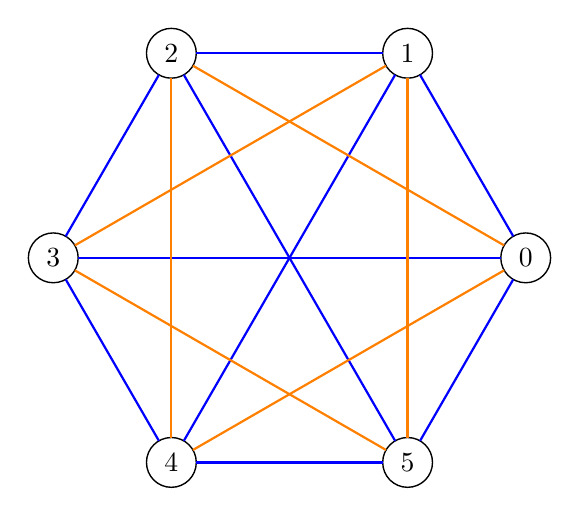
\begin{tikzpicture}
  \SetGraphUnit{3}
  \SetUpEdge[color = blue]
  \Vertices{circle}{0, 1, 2, 3, 4, 5}
  \Edges(0, 1, 2, 3, 4, 5, 0)
  \Edges(0, 3)
  \Edges(1, 4)
  \Edges(2, 5)
  \SetUpEdge[color = orange]
  \Edges(0, 2, 4, 0)
  \Edges(1, 3, 5, 1)
\end{tikzpicture}
\end{center}

Supoose we have a monochromatic triangle \(i < j < k\), then \(j - i, k - j, k - i\) are in the same part with \((k - j) + (j - i) = k - i\). This turns out to be exactly the setting we need to solve this problem. We will do this in chapter 1, alongside building the machinary we need.

\iffalse


Revision of \(\bigO\) notation and its cousins: let \(f,g:\N\to (0,\infty)\). We say
\begin{align*}
  f &= \bigO(g) \text{ if } f< Ag \text{ for some constant } A \\
  f &= \Omg(g) \text{ if } g=\bigO(f) \\
  f &= \bigT(g) \text{ if } f=\bigO(g) \text{ and } f = \Omg(g).
\end{align*}
Also,
\begin{align*}
  f &= \smallo(g) \text{ if } f/g\to 0 \text{ as } n\to \infty \\
  f &= \smallomg(g) \text{ if } f/g\to \infty \\
  f &\sim g \text{ if } f/g\to 1.
\end{align*}


\fi


\section{Extremal graph theory}

\subsection{Ramsey Theory}

\begin{definition}[graph, vertex, edge]\index{graph}
  A \emph{graph} \(G\) is an ordered pair \(G = (V, E)\) where \(V\) is a finite set and \(E\) is a set of unordered pairs of distinct elements of \(V\). The elements of \(V\) are the \emph{vertices} of \(G\) and those of \(E\) the \emph{edges}. Write \(V = V(E)\) and \(E = E(G)\).
\end{definition}

\begin{eg}
  \(G = ([9], \{12, 13, 14, 23, 67, 68, 69\})\). We often use picture to represent a graph.
  \begin{center}
    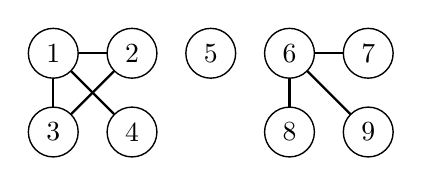
\begin{tikzpicture}
      \SetGraphUnit[3]
      \Vertex{1}
      \Vertex[x=1,y=0]{2}
      \Vertex[x=0,y=-1]{3}
      \Vertex[x=1,y=-1]{4}
      \Edges(1, 2, 3, 1)
      \Edges(1, 4)

      \Vertex[x=2,y=0]{5}

      \Vertex[x=3,y=0]{6}
      \Vertex[x=4,y=0]{7}
      \Vertex[x=3,y=-1]{8}
      \Vertex[x=4,y=-1]{9}
      \Edges(8,6,7)
      \Edges(6,9)
    \end{tikzpicture}
  \end{center}
\end{eg}

\begin{notation}
  We denote the edge \(\{i, j\}\) by \(ij\).
\end{notation}

\begin{eg}
  The \emph{complete graph of order \(n\)} \(K_n\) has \(V[K_n] = [n]\) and \(E(K_n) = \{ij: 1 \leq i < j \leq n\}\). For example, \(K_3\) is the \emph{triangle}\index{triangle}.
  \begin{center}
    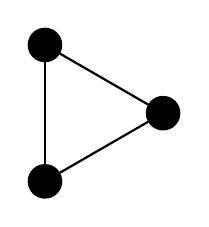
\begin{tikzpicture}
      \GraphInit[vstyle=Classic]
      \Vertices[NoLabel]{circle}{1, 2, 3}
      \Edges(1, 2, 3, 1)
    \end{tikzpicture}

    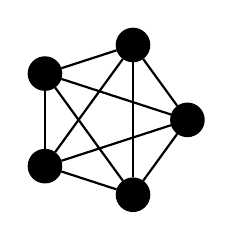
\begin{tikzpicture}
      \GraphInit[vstyle=Classic]
      \Vertices[NoLabel]{circle}{1, 2, 3, 4, 5}
      \Edges(1, 2, 3, 4, 5, 1, 3, 5, 2, 4, 1)
    \end{tikzpicture}
  \end{center}
\end{eg}

\begin{definition}[isomorphism]\index{isomorphism}
  An \emph{isomorphism} from a graph \(G\) to a graph \(H\) is a bijection \(\phi: V(G) \to V(H)\) satisfying \(\phi(u) \phi(v) \in E(H)\) if and only if \(uv \in E(G)\). If such \(\phi\) exists, we say \(G\) and \(H\) are \emph{isomorphic} and write \(G \cong H\).
\end{definition}

\begin{definition}[subgraph]\index{subgraph}
  A graph \(H\) is a \emph{subgraph} of a graph \(G\) if \(V(H) \subseteq V(G)\) and \(E(H) \subseteq E(G)\).

  More loosely, we \(H\) is a subgraph of \(G\) is \(H \cong H'\) for some subgraph \(H'\) of \(G\).

  Write \(H \subseteq G\) to mean \(H\) is a subgraph of \(G\).
\end{definition}

\begin{notation}
  Write \(v \in G\) to mean \(v \in V(G)\).
\end{notation}

\begin{definition}[colouring]\index{colouring}
  A \emph{\(k\)-colouring} of a graph \(G\) is a function \(c: E(G) \to [k]\).
\end{definition}

In proofs, if \(K\) is small, we often call colours blue, yellow, etc.\ rather than \(1, 2, \dots\).

\begin{definition}[monochromatic]\index{monochromatic}
  If \(G\) is \(k\)-coloured and \(H \subseteq G\), we say \(H\) is \emph{monochromatic} if \(c|_{E(H)}\) is constant.
\end{definition}

Now we are ready to tackle the colouring problem in the previous chapter.

\begin{eg}
  Suppose \(K_6\) is coloured blue/yellow. Pick \(v \in K_6\). \(v\) has \(5\) edges so some \(3\) are the same colour, wlog blue \(vw, vx, vy\). If any of \(wx, wy, xy\) is blue then we have a blue triangle. Otherwise \(wxy\) is a yellow triangle. Done.
\end{eg}

\begin{note}
  Note that it doesn't work in \(K_5\), i.e.\ \(K_5\) can be \(2\)-coloured with no monochromatic triangle:
  \begin{center}
    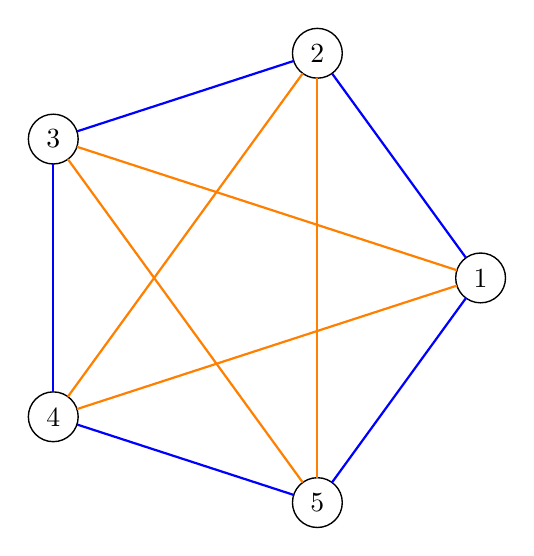
\begin{tikzpicture}
      \SetGraphUnit{3}
      \Vertices{circle}{1, 2, 3, 4, 5}
      \SetUpEdge[color = blue]
      \Edges(1,2,3,4,5,1)
      \SetUpEdge[color = orange]
      \Edges(1,3,5,2,4,1)
    \end{tikzpicture}
  \end{center}
\end{note}

\begin{proposition}[Ramsey's Theorem for triangles]\index{Ramsey's Theorem}
  Let \(k \in \N\). Then for \(n\) sufficiently large, if \(K_n\) is \(k\)-coloured we must have a monochromatic triangle.
\end{proposition}

\begin{proof}
  Induction on \(k\). For \(k = 1\), \(n = 3\) works. For \(k > 1\), by induction hypothesis we can choose \(m\) such that if \(K_m\) is \((k - 1)\)-coloured then it has a monochromatic triangle. Now take \(n = k(m - 1) + 2\). Suppose \(K_n\) is \(k\)-coloured. Pick \(v \in K_n\). There are \(k(m - 1) + 2\) edges from \(v\) so some \(m\) are the same colour. wlog \(v\) is joint to a \(K_m\), \(H\), by blue edegs. If \(H\) contains a blue edge then we have a blue triangle with \(v\). If not then \(H\) is a \((k - 1)\)-coloured \(K_m\) so by definition of \(m\) it contains a monochromatic triangle.
\end{proof}

\begin{remark}
  How big should we take \(n\)? Write \(f(k)\) for the smallest \(n\) that works. Then \(f(1) = 3\). If \(k > 1\), the proof tells us that \(f(k) \leq k(f(k - 1) - 1) + 2 \leq k f(k - 1)\). So by induction \(f(k) \leq 3k!\).
\end{remark}










\clearpage


\begin{question}
  How large must \(n\) be so that if edges of \(K_n\) are coloured blud and yellow then we always get mono \(K_s\)?
\end{question}

Let \(G\) be ``blue subgraph'' of \(K_n\), i.e. all vertices, only blue edges.
\begin{align*}
  K_n \text{ has a blue } K_s &\Leftrightarrow K_s \subseteq G \\
  K_n \text{ has a yellow } K_s &\Leftrightarrow G \text{ has an induced } \stcomp{K_s} \text{ subgraph}
\end{align*}

Rephrase: how large must \(n\) be to force every graph of order \(n\) to have \(K_s\) or \(\stcomp{K_s}\) as an induced subgraph?

This is a typical example of an \emph{extremal problem}: how large must some parameter of \(G\) be to force \(G\) to have a certain property?

Alternatively, how big can the parameter be with \(G\) not having the property?

\subsection{The Forbidden Subgraph Problem}

Fix a graph \(H\) with at least one edge. Let \(n \geq |H|\). Clealy \(H \subseteq K_n\) but \(H \nsubseteq \stcomp{K_n}\). How many edges must a graph \(G\) of order \(n\) have to force \(H \subseteq G\)? Alternatively, if \(|G| = n\) and \(H \nsubseteq G\), how large can \(e(G)\) be?

\begin{definition}
  Define
  \[
    \exx(n,H) := \max\{ e(G): |G|=n, H \nsubseteq G\}.
  \]
\end{definition}

\begin{question}
  Can we determine \(\exx(n,H)\)?
\end{question}

\subsubsection{Triangles}

Let \(H = K_3\). Want \(G\) with \(|G| = n\), \(e(G)\) large, \(\triangle \nsubseteq G\). Try partitioning \(V(G) = X\cup Y\) with all edges going from \(X\) to \(Y\).

\begin{definition}[Bipartite graph]
  A graph \(G\) is \emph{bipartite} (with bipartition \((X,Y)\)) if \(V(G)\) can be partitioned as \(X\cup Y\) in such a way that if \(e\in E(G)\) then \(e=xy\) for some \(x\in X, y\in Y\).
\end{definition}

Bipartite graphs have no \(\triangle\) (and indeed no cycles of odd length). In fact, the converse if true:

\begin{theorem}
  A graph is bipartite if and only if it contain no odd cycles.
\end{theorem}

\begin{proof}
  Later. Or exercise if you're ambitious.
\end{proof}

\begin{question}
  Which bipartite graph is the best?
\end{question}

Clearly want to include all possible edges from \(X\) to \(Y\).

\begin{definition}[Complete bipartite graph]
  Let \(s,t\geq 1\). The \emph{complete bipartite graph} \(K_{s,t}\) has bipartition \((X,Y)\) with \(|X| = s, |Y| = t\) and \(xy \in E(K_{s,t})\) for all \(x\in X, y\in Y\).
\end{definition}

We have
\begin{align*}
  |K_{s,t}| &= s+t \\
  e(K_{s,t}) &= st
\end{align*}
We want to maximise \(st\) subject to \(s+t=n\), i.e. maximise \(s(n-s)\), which is a quadratic in \(s\). So the best bipartite graph is
\[
  K_{\floor*{\frac{n}{2}}, \ceil*{\frac{n}{2}}}.
\]
But what if some \emph{non-bipartite} graph is better? For example, \(G\) is not bipartite but \(\triangle \nsubseteq G\) so \(e(K_{3,2}) = 6 > 5 = e(G)\). It turns out we don't have to worry: bipartite graph always wins.

\begin{theorem}[Mantel's Theorem]
  Let \(n\geq 3\). Suppose \(|G| = n, e(G) \geq \floor*{\frac{n^2}{4}}\) and \(\triangle \nsubseteq G\). Then
  \[
    G \cong K_{\floor*{\frac{n}{2}}, \ceil*{\frac{n}{2}}}.
  \]
\end{theorem}

\begin{proof}
  Proceed by induction on \(n\): if \(n=3\), there is only one possibility: \(G = K_{2,1}\). For \(n>3\), first remove edges from \(G\) if necessary to get \(H\) with \(|H| = n, e(H) = \floor*{\frac{n^2}{4}}\). Clearly \(\triangle \nsubseteq H\). Let \(v\in H\) with \(d(v) = \delta(H)\) and let \(K = H-v\). In other words, \(H\) with vertex \(v\) and all edges including \(v\) removed. Now \(|K| = n-1, \triangle \nsubseteq K\) and \(e(K) = \floor*{\frac{n^2}{4}} - \delta(H)\).

  Suppose \(n\) is even. Then
  \[
    \delta(H) \leq \text{average degree of } H = \frac{2e(H)}{|H|} = \frac{n^2/2}{n} = \frac{n}{2}.
  \]
  Hence \(e(K) \geq \frac{n^2}{4} - \frac{n}{2} = \frac{(n-1)^2}{4}-\frac{1}{4} = \floor*{\frac{(n-1)^2}{4}}\).

  Similarly if \(n\) is odd, also get \(e(K) \geq \floor*{\frac{(n-1)^2}{4}}\). Hence by induction hypothesis
  \[
    K \cong K_{\frac{n-1}{2},\frac{n-1}{2}}
  \]

  Also \(d(v) = e(H) - e(K)\) so if \(n\) is even
  \[
    d(v) = \frac{n^2}{4} - \frac{n^2-2n}{4} = \frac{n}{2}.
  \]
  \(H\) is formed by adding a vertex \(v\) to \(K \cong K_{\frac{n}{2},\frac{n-2}{2}}\), and joining \(v\) to \(\frac{n}{2}\) vertices of \(K_1\) without creating a \(\triangle\). If \(K\) has biparition \((X,Y)\), \(v\) cannot be joined both to vertex in \(X\) and vertex in \(Y\) so \(v\) must be joined to all vertices in larger of \(X\) and \(Y\). Thus \(H \cong K_{\floor*{\frac{n}{2}},\ceil*{\frac{n}{2}}}\) (and similar if \(n\) is odd).

  We recover \(G\) by adding edges to \(H\) without making a \(\triangle\). But any new edge creates a \(\triangle\). So \(G \cong H\).
\end{proof}

Hence if \(|G|=n, e(G) > floor \frac{n^2}{4}\) then \(G\) contains a \(\triangle\). Therefore \(\exx(n, \triangle) = \floor*{\frac{n^2}{4}}\).


\printindex
\end{document}
